\section{Foreseen product specifications}
\label{sec:org31f7574}
\subsection{QFD - Quality Function Deployment}

The use of a QFD "Quality House" was opted as it is an efficient method of defining requirements laid out for the project and convert them into somewhat detailed engineering specifications in order to fullfill those requirements, along with several tools that allow to define the relations existing between the latter and the former.

The QFD works by using a matrix where the project requirements will be laid out as rows and the engineering specifications as columns; in the intersections lie a number representing the strength of the relationship requirement-specification.

Along with the requirements, the importance given to each is also specified, ranging from 1 (lowest importance) to 5 (highest importance) these, along with the number at each intersection, will be used to calculate the Weighted Score of each requirement and the Technical Importance Score of each specification. These results will in turn be used to calculate the importance of each specification and thus assign priorities for the Design Team.

Figure ~\ref{fig:QFD} shows the "Quality House" for the RF CAR containing:
\begin{itemize}
\item Customer Requirements: Safe to Operate, Obstacle Avoidant, Fast, and so on.
\item Functional Requirements: Cost of Production, Maximum Velocity, Engine Power, amongst others.
\item The Intersection Values (referencing the strength of the requirement-specification correlation): 
\begin{itemize}
\item 0-No Relation.
\item 1-Weak Relation.
\item 3-Moderate Relation.
\item 9-Strong Relation.
\end{itemize}
\item The Analytical Results, depicting, quantifiably, the relevance of each entity:
\begin{itemize}
\item Weighted Score, for the Requirements.
\item Technical Importance Score, for the Specifications.
\item Importance and Priority Rank, which are the main conclusion for which the QFD was used.  
\end{itemize}
\end{itemize}
For instance: The "engine power" specification and the "fast" requirement have a very strong correlation (9) since the power of the engine is directly responsible for the velocity of the car. 

\begin{sidewaysfigure}[!htbp]
\centering
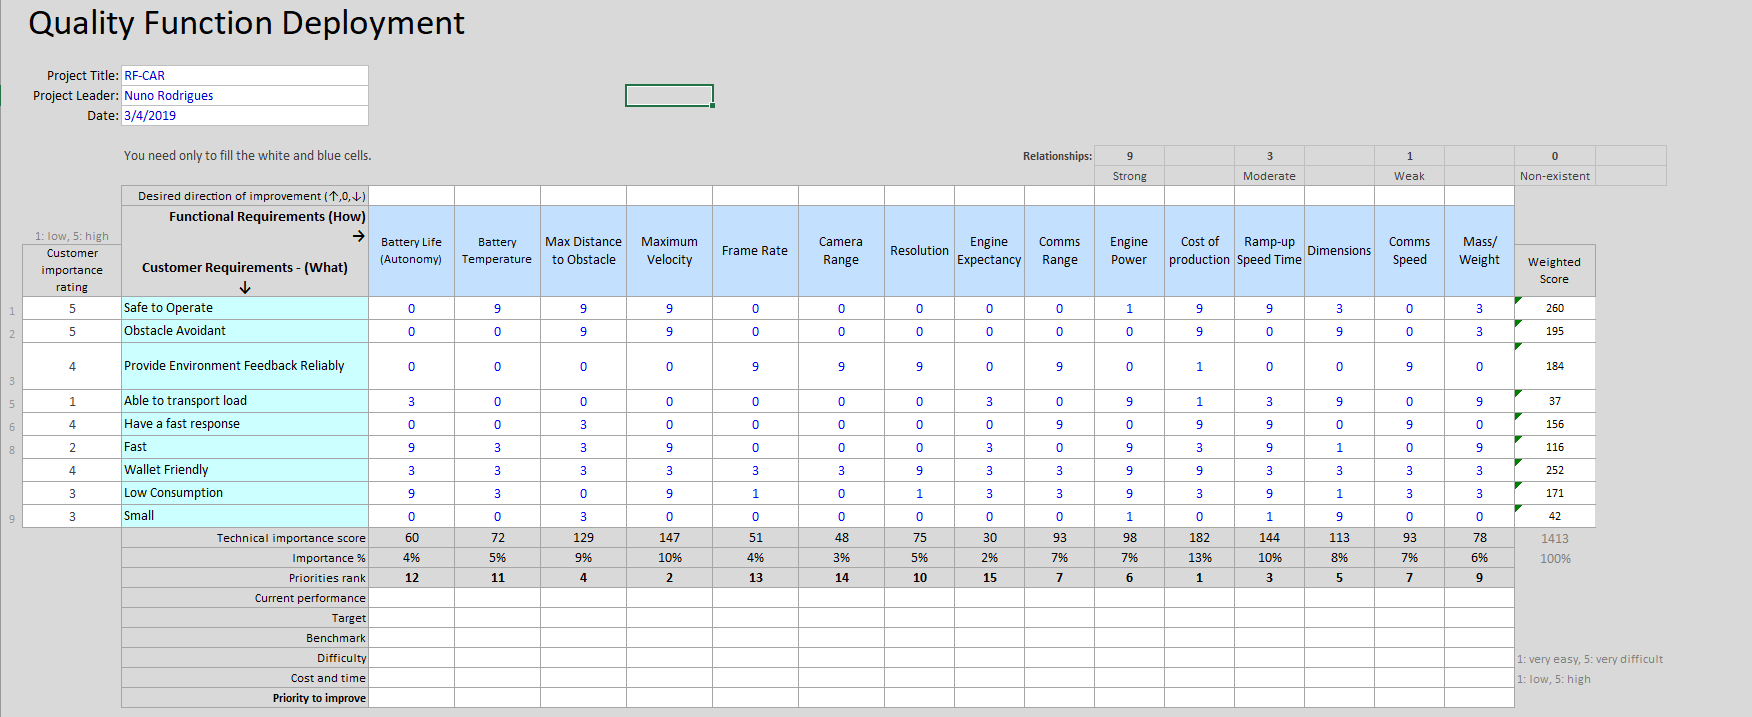
\includegraphics[width=1.25\textwidth]{./sec/img/QFD_Initial.png}
\caption{\label{fig:QFD}Foreseen product specifications:Quality Function Deployment for the RFCAR}
\end{sidewaysfigure}
\newpage
The foreseen product specifications are listed as topics below.

\subsection{Autonomy}
\label{sec:org7364ba5}
The vehicle is operated off-the-grid, thus, a portable power source must be included. The autonomy referes to the time interval between battery fully charged and safely discharged and should be observed for the following scenarios:
\begin{itemize}
\item No load;
\item Vehicle operating at maximum speed;
\item Vehicle operating at minimum speed.
\end{itemize}
\subsection{Velocity}
\label{sec:org08718bc}
The vehicle must be operated within a safe range of velocity, while also not increasing excessively the power consumption. Thus, these velocity boundaries should be tested in the absence of an external load and in the presence of the maximum load.
\subsection{Safety}
\label{sec:org83942c3}
For a remote controlled car, safety concerns not only the car itself and all of the equipment, but also the humans that interact with the car:
\begin{itemize}
\item Car: If the user issues a command that would cause damage to the system, the
system should take corrective measures to prevent it. The same holds true if
the communication between user and system is lost. The system uses odometric navigation.
\item Human: Due to the odometric sensors safely fixed in the car, crashes will not occur, making it much harder for the car to hit a person or for any part of the car to jump and cause harm to the user or anyone around.
\end{itemize}
\subsection{Image acquisition}
\label{sec:orgb6a5f66}
\subsubsection{Frame rate}
\label{sec:org5adf4ee}
Frame rate refers to the frequency at which independent still images appear on the screen. The higher the frame rate, a better image quality is obtained but the processing overhead increases as well, so a compromise must be achieved between the quality of the image and the processing overhead required. The minimum frame rate defined must be such that allows a clear view of the video.
\subsubsection{Range}
\label{sec:orgecb044c}
How far can the camera capture images without loosing resolution and record them. The range must such that allows the user to see the obstacles when the car is heading to them and provide enough time to change the direction.
\subsubsection{Resolution}
\label{sec:orgba87554}
The amount of detail that the camera can capture. It is measured in pixels. The quality of the aquired image is proportional to the number os pixels but a greater resolution requires a greater data transfer and processing overhead, thus, a compromise must be achieved. The minimum resolution must be such that provides the least amount of information required for the user. 
\subsection{Load}
\label{sec:orgca6a690}
The remotely controlled vehicle can be used in applications involving load carrying (besides its own), e.g., packet delivery. For this purpose it is important to determine the maximum load the vehicle can carry safely at the minimum velocity defined. As the load increases, also increases the power consumption, diminishing the autonomy.
\subsection{Overall System latency/responsivess}
\label{sec:org7fd1829}
The overall system latency is the sum of all systems' latencies, which must be under a maximum tolerated value for the user.
\subsection{Communication}
\label{sec:org4241610}
\subsubsection{Reliability}
\label{sec:orgdcb920d}
A communication is reliable if it guarantees measures to deliver the data conveyed in the communication link. As reliability imposes these measures, it also adds overhead to the communication protocol, which must be considered depending on the case. For example, for the devised product, an user command must be acknowledged to be processed, otherwise, the user must be informed; on the other hand, loosing frames from the video feed is not so critical — user can still observe conveniently the field of vision if the frame rate is within acceptable boundaries.
\subsubsection{Range}
\label{sec:org447a205}
The communication protocols have a limited range of operation, and, as such, regarding the environment on which the car is used the range can be changed.
The range refers to the maximum distance allowed between user and system for communication purposes.
\subsection{Sensibility}
\label{sec:org622e63a}
The movement of the car will be determined by the tilt movement of the smartphone. Sensibility refers to the responsiveness of the car on the minimum smartphone tilt movement. The sensibility must be in an range of values in which small unintentional movements will be enough to change the state of the car and it does not take big smartphone tilts for the car to move.
\subsection{Closed loop error}
\label{sec:org436f732}
The velocity, direction and distance to obstacles must be continuosly monitored to ensure proper vehicle operation. The closed loop error must then be checked mainly in three situations as a response to an user command:
\begin{itemize}
\item velocity: the user issued an command with a given mean velocity, which should be compared with the steady-state mean velocity of the vehicle.
\item direction: the user issued an command with a given direction, which should be compared to the vehicle direction.
\item distance to obstacles: the user issued an command with a given direction and velocity which can cause it to crash. The local control must take over control, preventing this to happen, and the final distance to the obstacles must be assessed and compared to the defined one.
\end{itemize}
\subsection{Summary}
\label{sec:org1f95256}
Table \ref{tab:specs-init} lists the foreseen product specifications.

% Please add the following required packages to your document preamble:
% \usepackage[table,xcdraw]{xcolor}
% If you use beamer only pass "xcolor=table" option, i.e. \documentclass[xcolor=table]{beamer}
% Please add the following required packages to your document preamble:
% \usepackage[table,xcdraw]{xcolor}
% If you use beamer only pass "xcolor=table" option, i.e. \documentclass[xcolor=table]{beamer}
\begin{table}[!hbt]
\centering
\caption{Specifications}
\label{tab:specs-init}

\begin{tabular}{
>{\columncolor[HTML]{FFFFFF}}l 
>{\columncolor[HTML]{FFFFFF}}l 
>{\columncolor[HTML]{FFFFFF}}l }
\hline
                  & Values     & Explanation                                                                                                  \\ \hline
Autonomy          & 4 h        & \begin{tabular}[c]{@{}l@{}}Time interval between battery fully \\ charged and safely discharged\end{tabular} \\ \hline
Minimum Velocity  & 0.1 m/s    & \begin{tabular}[c]{@{}l@{}}Minimum velocity at which the car \\ can operate safely\end{tabular}              \\ \hline
Maximum Velocity  & 1 m/s      & \begin{tabular}[c]{@{}l@{}}Maximum velocity at which the car\\ can operate safely\end{tabular}               \\ \hline
Maximum Load      & 0.5 kg     & Maximum load the car can safely carry                                                                        \\ \hline
Frame Rate        & 60 fps     & \begin{tabular}[c]{@{}l@{}}Frequency at which independent still \\ images appear on the screen\end{tabular}  \\ \hline
Camera Range      & 20 m       & \begin{tabular}[c]{@{}l@{}}How far can the camera capture images\\ without loosing resolution\end{tabular}   \\ \hline
Camera resolution & 480p       & Amount of detail that the camera can capture                                                                 \\ \hline
Comunication Range & 50 m & \begin{tabular}[c]{@{}l@{}}Maximum distance between the car and the\\ smarphone without losing connection\end{tabular} \\ \hline
Velocity Error    & 5 \%       & \begin{tabular}[c]{@{}l@{}}Maximum difference between desired \\ and real velocity\end{tabular}              \\ \hline
Direction Error   & 5\%        & \begin{tabular}[c]{@{}l@{}}Maximum difference between desired\\  and real direction\end{tabular}             \\ \hline
Distance Error     & 5 \% & \begin{tabular}[c]{@{}l@{}}Maximum difference between desired\\ and real distance to the obstacle\end{tabular}         \\ \hline
Dimensions        & 20x12x5 cm & Dimensions of the car                                                                                        \\ \hline
Weight            & 0.5 kg     & Weight of the car                                                                                            \\ \hline
\end{tabular}
\end{table}

%%% Local Variables:
%%% mode: latex
%%% TeX-master: "../Phase1"
%%% End:
